\chapter{Dinamičko programiranje}

\index{dinamičko programiranje}

\key{Dinamičko programiranje}
je tehnika koja spaja točnost
potpune pretrage i efikasnost
pohlepnih algoritama.
Dinamičko programiranje možemo primijeniti ako se
zadatak može podijeliti na preklapajuće potprobleme
koji se mogu rješavati neovisno.

Postoje dvije primjene dinamičkog programiranja:

\begin{itemize}
\item
\key{Pronalaženje optimalnog rješenja}:
Želimo pronaći rješenje koje je
što veće ili što manje.
\item
\key{Brojanje broja rješenja}:
Želimo izračunati ukupan broj
mogućih rješenja.
\end{itemize}

Najprije ćemo vidjeti kako se dinamičko programiranje
može upotrijebiti za pronalaženje optimalnog rješenja,
a zatim ćemo istu ideju iskoristiti za
brojanje rješenja.

Razumijevanje dinamičkog programiranja prekretnica je
u karijeri svakog natjecateljskog programera.
Iako je osnovna ideja jednostavna,
izazov je kako primijeniti
dinamičko programiranje na različite zadatke.
Ovo poglavlje uvodi skup klasičnih zadataka
koji su dobra polazna točka.

\section{Zadatak s kovanicama}

Najprije se usredotočimo na zadatak koji smo
već vidjeli u poglavlju 6:
Zadan je skup vrijednosti kovanica $\texttt{coins} = \{c_1,c_2,\ldots,c_k\}$
i ciljni iznos novca $n$, a naš je zadatak
oblikovati sumu $n$ koristeći što manje kovanica.

U poglavlju 6 taj smo zadatak riješili
pohlepnim algoritmom koji uvijek bira najveću
moguću kovanicu.
Pohlepni algoritam radi, na primjer,
kada su kovanice euro kovanice,
ali u općem slučaju pohlepni algoritam
ne daje nužno optimalno rješenje.

Sada je vrijeme da zadatak riješimo efikasno
pomoću dinamičkog programiranja, tako da algoritam
radi za bilo koji skup kovanica.
Algoritam dinamičkog programiranja
temelji se na rekurzivnoj funkciji
koja prolazi kroz sve mogućnosti kako
oblikovati sumu, poput algoritma grube sile.
Međutim, algoritam dinamičkog programiranja
je efikasan jer
koristi \emph{memoizaciju} i
odgovor na svaki potproblem izračunava samo jednom.

\subsubsection{Rekurzivna formulacija}

Ideja dinamičkog programiranja jest
formulirati zadatak rekurzivno tako
da se rješenje zadatka može
izračunati iz rješenja manjih
potproblema.
U zadatku s kovanicama prirodan rekurzivni
zadatak glasi ovako:
koji je najmanji broj kovanica
potreban za oblikovanje sume $x$?

Neka $\texttt{solve}(x)$
označava najmanji
broj kovanica potreban za sumu $x$.
Vrijednosti funkcije ovise o
vrijednostima kovanica.
Na primjer, ako je $\texttt{coins} = \{1,3,4\}$,
prve vrijednosti funkcije su sljedeće:

\[
\begin{array}{lcl}
\texttt{solve}(0) & = & 0 \\
\texttt{solve}(1) & = & 1 \\
\texttt{solve}(2) & = & 2 \\
\texttt{solve}(3) & = & 1 \\
\texttt{solve}(4) & = & 1 \\
\texttt{solve}(5) & = & 2 \\
\texttt{solve}(6) & = & 2 \\
\texttt{solve}(7) & = & 2 \\
\texttt{solve}(8) & = & 2 \\
\texttt{solve}(9) & = & 3 \\
\texttt{solve}(10) & = & 3 \\
\end{array}
\]

Na primjer, $\texttt{solve}(10)=3$,
jer su potrebne barem 3 kovanice
da bi se oblikovala suma 10.
Optimalno rješenje je $3+3+4=10$.

Bitno svojstvo funkcije $\texttt{solve}$ jest
da se njezine vrijednosti mogu
rekurzivno izračunati iz njezinih manjih vrijednosti.
Ideja je usredotočiti se na \emph{prvu}
kovanicu koju biramo za sumu.
Na primjer, u gornjem scenariju
prva kovanica može biti 1, 3 ili 4.
Ako najprije odaberemo kovanicu 1,
preostali zadatak je oblikovati sumu 9
koristeći najmanji broj kovanica,
što je potproblem izvornog zadatka.
Naravno, isto vrijedi za kovanice 3 i 4.
Stoga možemo koristiti sljedeću rekurzivnu formulu
za izračun najmanjeg broja kovanica:
\begin{equation*}
\begin{split}
\texttt{solve}(x) = \min( & \texttt{solve}(x-1)+1, \\
                           & \texttt{solve}(x-3)+1, \\
                           & \texttt{solve}(x-4)+1).
\end{split}
\end{equation*}
Bazni slučaj rekurzije je $\texttt{solve}(0)=0$,
jer za oblikovanje prazne sume nije potrebna nijedna kovanica.
Na primjer,
\[ \texttt{solve}(10) = \texttt{solve}(7)+1 = \texttt{solve}(4)+2 = \texttt{solve}(0)+3 = 3.\]

Sada smo spremni napisati opću rekurzivnu funkciju
koja izračunava najmanji broj
kovanica potreban za oblikovanje sume $x$:
\begin{equation*}
    \texttt{solve}(x) = \begin{cases}
               \infty               & x < 0\\
               0               & x = 0\\
               \min_{c \in \texttt{coins}} \texttt{solve}(x-c)+1 & x > 0 \\
           \end{cases}
\end{equation*}

Prvo, ako je $x<0$, vrijednost je $\infty$,
jer je nemoguće oblikovati negativnu
sumu novca.
Zatim, ako je $x=0$, vrijednost je $0$,
jer za oblikovanje prazne sume nije potrebna nijedna kovanica.
Konačno, ako je $x>0$, varijabla $c$ prolazi kroz
sve mogućnosti kako odabrati prvu kovanicu
sume.

Kada smo pronašli rekurzivnu funkciju koja rješava
zadatak,
možemo izravno implementirati rješenje u C++-u
(konstanta \texttt{INF} označava beskonačnost):

\begin{lstlisting}
int solve(int x) {
    if (x < 0) return INF;
    if (x == 0) return 0;
    int best = INF;
    for (auto c : coins) {
        best = min(best, solve(x-c)+1);
    }
    return best;
}
\end{lstlisting}

Ipak, ova funkcija nije efikasna,
jer može postojati eksponencijalan broj načina
za konstrukciju sume.
Međutim, sljedeće ćemo vidjeti kako funkciju
učiniti efikasnom pomoću tehnike zvane memoizacija.

\subsubsection{Korištenje memoizacije}

\index{memoizacija}

Ideja dinamičkog programiranja jest koristiti
\key{memoizaciju} za efikasan izračun
vrijednosti rekurzivne funkcije.
To znači da se vrijednosti funkcije
nakon izračuna pohranjuju u niz.
Za svaki parametar vrijednost funkcije
izračunava se rekurzivno samo jednom, a nakon toga
vrijednost se može izravno dohvatiti iz niza.

U ovom zadatku koristimo nizove
\begin{lstlisting}
bool ready[N];
int value[N];
\end{lstlisting}

gdje $\texttt{ready}[x]$ označava
je li vrijednost $\texttt{solve}(x)$ izračunata,
a ako jest, $\texttt{value}[x]$
sadrži tu vrijednost.
Konstanta $N$ odabrana je tako
da sve potrebne vrijednosti stanu u nizove.

Sada se funkcija može efikasno
implementirati ovako:

\begin{lstlisting}
int solve(int x) {
    if (x < 0) return INF;
    if (x == 0) return 0;
    if (ready[x]) return value[x];
    int best = INF;
    for (auto c : coins) {
        best = min(best, solve(x-c)+1);
    }
    value[x] = best;
    ready[x] = true;
    return best;
}
\end{lstlisting}

Funkcija obrađuje bazne slučajeve
$x<0$ i $x=0$ kao i prije.
Zatim funkcija iz
$\texttt{ready}[x]$ provjerava je li
$\texttt{solve}(x)$ već pohranjen
u $\texttt{value}[x]$,
i ako jest, funkcija ga izravno vraća.
Inače funkcija rekurzivno izračunava vrijednost
$\texttt{solve}(x)$
i pohranjuje je u $\texttt{value}[x]$.

Ova funkcija radi efikasno,
jer se odgovor za svaki parametar $x$
izračunava rekurzivno samo jednom.
Nakon što je vrijednost $\texttt{solve}(x)$ pohranjena u $\texttt{value}[x]$,
može se efikasno dohvatiti kad god se
funkcija ponovno pozove s parametrom $x$.
Vremenska složenost algoritma je $O(nk)$,
gdje je $n$ ciljna suma, a $k$ broj kovanica.

Primijetimo da niz \texttt{value} možemo
konstruirati i \emph{iterativno} koristeći
petlju koja jednostavno izračunava sve vrijednosti
funkcije $\texttt{solve}$ za parametre $0 \ldots n$:
\begin{lstlisting}
value[0] = 0;
for (int x = 1; x <= n; x++) {
    value[x] = INF;
    for (auto c : coins) {
        if (x-c >= 0) {
            value[x] = min(value[x], value[x-c]+1);
        }
    }
}
\end{lstlisting}

Zapravo, većina natjecateljskih programera preferira ovu
implementaciju, jer je kraća i ima
manje konstantne faktore.
Od sada i mi u našim primjerima koristimo
iterativne implementacije.
Ipak, često je lakše razmišljati o
rješenjima dinamičkog programiranja
u terminima rekurzivnih funkcija.


\subsubsection{Konstrukcija rješenja}

Ponekad se od nas traži i da pronađemo vrijednost
optimalnog rješenja i da damo
primjer kako se takvo rješenje može konstruirati.
U zadatku s kovanicama, na primjer,
možemo deklarirati još jedan niz
koji za svaku sumu novca
označava prvu kovanicu
u optimalnom rješenju:
\begin{lstlisting}
int first[N];
\end{lstlisting}
Zatim algoritam možemo izmijeniti ovako:
\begin{lstlisting}
value[0] = 0;
for (int x = 1; x <= n; x++) {
    value[x] = INF;
    for (auto c : coins) {
        if (x-c >= 0 && value[x-c]+1 < value[x]) {
            value[x] = value[x-c]+1;
            first[x] = c;
        }
    }
}
\end{lstlisting}
Nakon toga, sljedeći kod možemo koristiti za
ispis kovanica koje se pojavljuju u optimalnom rješenju za
sumu $n$:
\begin{lstlisting}
while (n > 0) {
    cout << first[n] << "\n";
    n -= first[n];
}
\end{lstlisting}

\subsubsection{Brojanje broja rješenja}

Razmotrimo sada drugu verziju
zadatka s kovanicama u kojoj je naš zadatak
izračunati ukupan broj načina
da se proizvede suma $x$ koristeći kovanice.
Na primjer, ako je $\texttt{coins}=\{1,3,4\}$ i
$x=5$, postoji ukupno 6 načina:

\begin{multicols}{2}
\begin{itemize}
\item $1+1+1+1+1$
\item $1+1+3$
\item $1+3+1$
\item $3+1+1$
\item $1+4$
\item $4+1$
\end{itemize}
\end{multicols}

Ponovno, zadatak možemo riješiti rekurzivno.
Neka $\texttt{solve}(x)$ označava broj načina
na koje možemo oblikovati sumu $x$.
Na primjer, ako je $\texttt{coins}=\{1,3,4\}$,
tada je $\texttt{solve}(5)=6$, a rekurzivna formula je
\begin{equation*}
\begin{split}
\texttt{solve}(x) = & \texttt{solve}(x-1) + \\
                    & \texttt{solve}(x-3) + \\
                    & \texttt{solve}(x-4)  .
\end{split}
\end{equation*}

Tada opća rekurzivna funkcija glasi ovako:
\begin{equation*}
    \texttt{solve}(x) = \begin{cases}
               0               & x < 0\\
               1               & x = 0\\
               \sum_{c \in \texttt{coins}} \texttt{solve}(x-c) & x > 0 \\
           \end{cases}
\end{equation*}

Ako je $x<0$, vrijednost je 0, jer nema rješenja.
Ako je $x=0$, vrijednost je 1, jer postoji samo jedan način
za oblikovanje prazne sume.
Inače izračunavamo sumu svih vrijednosti
oblika $\texttt{solve}(x-c)$ gdje je $c$ u \texttt{coins}.

Sljedeći kod konstruira niz
$\texttt{count}$ takav da je
$\texttt{count}[x]$ jednak
vrijednosti $\texttt{solve}(x)$
za $0 \le x \le n$:

\begin{lstlisting}
count[0] = 1;
for (int x = 1; x <= n; x++) {
    for (auto c : coins) {
        if (x-c >= 0) {
            count[x] += count[x-c];
        }
    }
}
\end{lstlisting}

Često je broj rješenja toliko velik
da nije potrebno izračunati točan broj,
nego je dovoljno dati odgovor modulo $m$
gdje je, na primjer, $m=10^9+7$.
To možemo postići izmjenom koda tako da se
svi izračuni obavljaju modulo $m$.
U gornjem kodu dovoljno je dodati redak
\begin{lstlisting}
        count[x] %= m;
\end{lstlisting}
nakon retka
\begin{lstlisting}
        count[x] += count[x-c];
\end{lstlisting}

Sada smo raspravili sve osnovne
ideje dinamičkog programiranja.
Budući da se dinamičko programiranje može koristiti
u mnogo različitih situacija,
sada ćemo proći kroz skup zadataka
koji pokazuju daljnje primjere
mogućnosti dinamičkog programiranja.

\section{Najdulji rastući podslijed}

\index{najdulji rastući podslijed}

Naš prvi zadatak je pronaći
\key{najdulji rastući podslijed}
u nizu od $n$ elemenata.
To je slijed elemenata niza
maksimalne duljine
koji ide slijeva nadesno,
i svaki element u slijedu veći je
od prethodnog elementa.
Na primjer, u nizu

\begin{center}
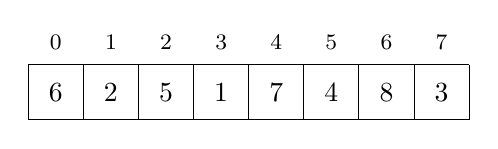
\begin{tikzpicture}[scale=0.7]
\draw (0,0) grid (8,1);
\node at (0.5,0.5) {$6$};
\node at (1.5,0.5) {$2$};
\node at (2.5,0.5) {$5$};
\node at (3.5,0.5) {$1$};
\node at (4.5,0.5) {$7$};
\node at (5.5,0.5) {$4$};
\node at (6.5,0.5) {$8$};
\node at (7.5,0.5) {$3$};

\footnotesize
\node at (0.5,1.4) {$0$};
\node at (1.5,1.4) {$1$};
\node at (2.5,1.4) {$2$};
\node at (3.5,1.4) {$3$};
\node at (4.5,1.4) {$4$};
\node at (5.5,1.4) {$5$};
\node at (6.5,1.4) {$6$};
\node at (7.5,1.4) {$7$};
\end{tikzpicture}
\end{center}
najdulji rastući podslijed
sadrži 4 elementa:
\begin{center}
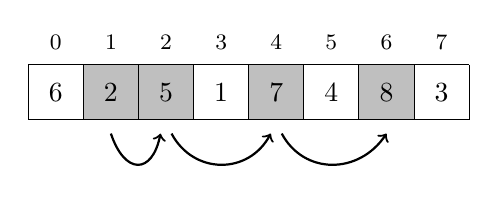
\begin{tikzpicture}[scale=0.7]
\fill[color=lightgray] (1,0) rectangle (2,1);
\fill[color=lightgray] (2,0) rectangle (3,1);
\fill[color=lightgray] (4,0) rectangle (5,1);
\fill[color=lightgray] (6,0) rectangle (7,1);
\draw (0,0) grid (8,1);
\node at (0.5,0.5) {$6$};
\node at (1.5,0.5) {$2$};
\node at (2.5,0.5) {$5$};
\node at (3.5,0.5) {$1$};
\node at (4.5,0.5) {$7$};
\node at (5.5,0.5) {$4$};
\node at (6.5,0.5) {$8$};
\node at (7.5,0.5) {$3$};

\draw[thick,->] (1.5,-0.25) .. controls (1.75,-1.00) and (2.25,-1.00) .. (2.4,-0.25);
\draw[thick,->] (2.6,-0.25) .. controls (3.0,-1.00) and (4.0,-1.00) .. (4.4,-0.25);
\draw[thick,->] (4.6,-0.25) .. controls (5.0,-1.00) and (6.0,-1.00) .. (6.5,-0.25);

\footnotesize
\node at (0.5,1.4) {$0$};
\node at (1.5,1.4) {$1$};
\node at (2.5,1.4) {$2$};
\node at (3.5,1.4) {$3$};
\node at (4.5,1.4) {$4$};
\node at (5.5,1.4) {$5$};
\node at (6.5,1.4) {$6$};
\node at (7.5,1.4) {$7$};
\end{tikzpicture}
\end{center}

Neka $\texttt{length}(k)$ označava
duljinu najduljeg
rastućeg podslijeda
koji završava na poziciji $k$.
Dakle, ako izračunamo sve vrijednosti
$\texttt{length}(k)$ gdje je $0 \le k \le n-1$,
saznat ćemo duljinu
najduljeg rastućeg podslijeda.
Na primjer, vrijednosti funkcije
za gornji niz su sljedeće:
\[
\begin{array}{lcl}
\texttt{length}(0) & = & 1 \\
\texttt{length}(1) & = & 1 \\
\texttt{length}(2) & = & 2 \\
\texttt{length}(3) & = & 1 \\
\texttt{length}(4) & = & 3 \\
\texttt{length}(5) & = & 2 \\
\texttt{length}(6) & = & 4 \\
\texttt{length}(7) & = & 2 \\
\end{array}
\]

Na primjer, $\texttt{length}(6)=4$,
jer se najdulji rastući podslijed
koji završava na poziciji 6 sastoji od 4 elementa.

Da bismo izračunali vrijednost $\texttt{length}(k)$,
trebamo pronaći poziciju $i<k$
za koju je $\texttt{array}[i]<\texttt{array}[k]$
i $\texttt{length}(i)$ je što veći.
Tada znamo da je
$\texttt{length}(k)=\texttt{length}(i)+1$,
jer je to optimalan način da se
$\texttt{array}[k]$ doda podslijedu.
Međutim, ako takva pozicija $i$ ne postoji,
tada je $\texttt{length}(k)=1$,
što znači da podslijed sadrži samo
$\texttt{array}[k]$.

Budući da se sve vrijednosti funkcije mogu izračunati
iz njezinih manjih vrijednosti,
možemo koristiti dinamičko programiranje.
U sljedećem kodu vrijednosti
funkcije bit će pohranjene u nizu
$\texttt{length}$.

\begin{lstlisting}
for (int k = 0; k < n; k++) {
    length[k] = 1;
    for (int i = 0; i < k; i++) {
        if (array[i] < array[k]) {
            length[k] = max(length[k],length[i]+1);
        }
    }
}
\end{lstlisting}

Ovaj kod radi u $O(n^2)$ vremenu,
jer se sastoji od dviju ugniježđenih petlji.
Međutim, izračun dinamičkog programiranja
moguće je implementirati
i efikasnije, u $O(n \log n)$ vremenu.
Možete li pronaći način kako to učiniti?

\section{Putovi u mreži}

Naš sljedeći zadatak je pronaći put
od gornjeg lijevog kuta do
donjeg desnog kuta
mreže $n \times n$, tako da se
krećemo samo prema dolje i udesno.
Svaki kvadrat sadrži pozitivan cijeli broj,
a put treba konstruirati tako
da suma vrijednosti duž
puta bude što veća.

Sljedeća slika prikazuje optimalan
put u mreži:
\begin{center}
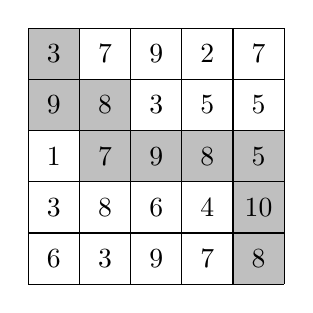
\begin{tikzpicture}[scale=.65]
  \begin{scope}
    \fill [color=lightgray] (0, 9) rectangle (1, 8);
    \fill [color=lightgray] (0, 8) rectangle (1, 7);
    \fill [color=lightgray] (1, 8) rectangle (2, 7);
    \fill [color=lightgray] (1, 7) rectangle (2, 6);
    \fill [color=lightgray] (2, 7) rectangle (3, 6);
    \fill [color=lightgray] (3, 7) rectangle (4, 6);
    \fill [color=lightgray] (4, 7) rectangle (5, 6);
    \fill [color=lightgray] (4, 6) rectangle (5, 5);
    \fill [color=lightgray] (4, 5) rectangle (5, 4);
    \draw (0, 4) grid (5, 9);
    \node at (0.5,8.5) {3};
    \node at (1.5,8.5) {7};
    \node at (2.5,8.5) {9};
    \node at (3.5,8.5) {2};
    \node at (4.5,8.5) {7};
    \node at (0.5,7.5) {9};
    \node at (1.5,7.5) {8};
    \node at (2.5,7.5) {3};
    \node at (3.5,7.5) {5};
    \node at (4.5,7.5) {5};
    \node at (0.5,6.5) {1};
    \node at (1.5,6.5) {7};
    \node at (2.5,6.5) {9};
    \node at (3.5,6.5) {8};
    \node at (4.5,6.5) {5};
    \node at (0.5,5.5) {3};
    \node at (1.5,5.5) {8};
    \node at (2.5,5.5) {6};
    \node at (3.5,5.5) {4};
    \node at (4.5,5.5) {10};
    \node at (0.5,4.5) {6};
    \node at (1.5,4.5) {3};
    \node at (2.5,4.5) {9};
    \node at (3.5,4.5) {7};
    \node at (4.5,4.5) {8};
  \end{scope}
\end{tikzpicture}
\end{center}
Suma vrijednosti na putu je 67,
i to je najveća moguća suma na putu
od
gornjeg lijevog kuta do donjeg desnog kuta.

Pretpostavimo da su redci i stupci
mreže numerirani od 1 do $n$,
a $\texttt{value}[y][x]$ jednak je vrijednosti
kvadrata $(y,x)$.
Neka $\texttt{sum}(y,x)$ označava najveću
sumu na putu od gornjeg lijevog kuta
do kvadrata $(y,x)$.
Sada nam $\texttt{sum}(n,n)$ govori
najveću sumu
od gornjeg lijevog kuta do
donjeg desnog kuta.
Na primjer, u gornjoj mreži
$\texttt{sum}(5,5)=67$.

Sume možemo rekurzivno izračunati
ovako:
\[ \texttt{sum}(y,x) = \max(\texttt{sum}(y,x-1),\texttt{sum}(y-1,x))+\texttt{value}[y][x]\]


Rekurzivna formula temelji se na zapažanju
da put koji završava u kvadratu $(y,x)$
može doći ili iz kvadrata $(y,x-1)$
ili iz kvadrata $(y-1,x)$:
\begin{center}
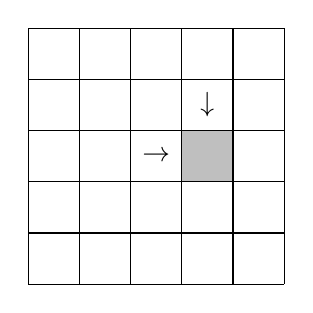
\begin{tikzpicture}[scale=.65]
  \begin{scope}
    \fill [color=lightgray] (3, 7) rectangle (4, 6);
    \draw (0, 4) grid (5, 9);
    
    \node at (2.5,6.5) {$\rightarrow$};
    \node at (3.5,7.5) {$\downarrow$};
    
  \end{scope}
\end{tikzpicture}
\end{center}

Dakle, biramo smjer koji maksimizira
sumu.
Pretpostavljamo da je $\texttt{sum}(y,x)=0$
ako je $y=0$ ili $x=0$ (jer takvi putovi ne postoje),
pa rekurzivna formula radi i kada je $y=1$ ili $x=1$.

Budući da funkcija \texttt{sum} ima dva parametra,
i niz dinamičkog programiranja ima dvije dimenzije.
Na primjer, možemo koristiti niz
\begin{lstlisting}
int sum[N][N];
\end{lstlisting}
i izračunati sume ovako:
\begin{lstlisting}
for (int y = 1; y <= n; y++) {
    for (int x = 1; x <= n; x++) {
        sum[y][x] = max(sum[y][x-1],sum[y-1][x])+value[y][x];
    }
}
\end{lstlisting}
Vremenska složenost algoritma je $O(n^2)$.

\section{Problemi ruksaka}

\index{ruksak}

Pojam \key{ruksak} odnosi se na zadatke u kojima je
zadan skup objekata, a treba
pronaći podskupove
s određenim svojstvima.
Problemi ruksaka često se mogu riješiti
dinamičkim programiranjem.

U ovom odjeljku usredotočujemo se na sljedeći
zadatak: Zadana je lista težina
$[w_1,w_2,\ldots,w_n]$,
odredite sve
sume koje se mogu konstruirati koristeći te težine.
Na primjer, ako su težine
$[1,3,3,5]$, moguće su sljedeće sume:

\begin{center}
\begin{tabular}{rrrrrrrrrrrrr}
 0 & 1 & 2 & 3 & 4 & 5 & 6 & 7 & 8 & 9 & 10 & 11 & 12 \\
\hline
 X & X & & X & X & X & X & X & X & X & & X & X \\
\end{tabular}
\end{center}

U ovom slučaju moguće su sve sume između $0 \ldots 12$,
osim 2 i 10.
Na primjer, suma 7 je moguća jer
možemo odabrati težine $[1,3,3]$.

Da bismo riješili zadatak, usredotočujemo se na potprobleme
u kojima za konstrukciju suma koristimo samo prvih $k$
težina.
Neka je $\texttt{possible}(x,k)=\textrm{true}$ ako
možemo konstruirati sumu $x$
koristeći prvih $k$ težina,
a inače $\texttt{possible}(x,k)=\textrm{false}$.
Vrijednosti funkcije mogu se rekurzivno
izračunati ovako:
\[ \texttt{possible}(x,k) = \texttt{possible}(x-w_k,k-1) \lor \texttt{possible}(x,k-1) \]
Formula se temelji na činjenici da težinu $w_k$
u sumi možemo ili iskoristiti ili ne iskoristiti.
Ako iskoristimo $w_k$, preostali zadatak je
oblikovati sumu $x-w_k$ koristeći prvih $k-1$ težina,
a ako ne iskoristimo $w_k$,
preostali zadatak je oblikovati sumu $x$
koristeći prvih $k-1$ težina.
Kao bazne slučajeve imamo
\begin{equation*}
    \texttt{possible}(x,0) = \begin{cases}
               \textrm{true}    & x = 0\\
               \textrm{false}   & x \neq 0 \\
           \end{cases}
\end{equation*}
jer ako se ne koristi nijedna težina,
možemo oblikovati samo sumu 0.

Sljedeća tablica prikazuje sve vrijednosti funkcije
za težine $[1,3,3,5]$ (simbol ''X''
označava vrijednosti true):

\begin{center}
\begin{tabular}{r|rrrrrrrrrrrrr}
$k \backslash x$ & 0 & 1 & 2 & 3 & 4 & 5 & 6 & 7 & 8 & 9 & 10 & 11 & 12 \\
\hline
 0 & X & \\
 1 & X & X \\
 2 & X & X & & X & X \\
 3 & X & X & & X & X & & X & X \\
 4 & X & X & & X & X & X & X & X & X & X & & X & X \\
\end{tabular}
\end{center}

Nakon izračuna tih vrijednosti, $\texttt{possible}(x,n)$
nam govori možemo li konstruirati
sumu $x$ koristeći \emph{sve} težine.

Neka $W$ označava ukupnu sumu težina.
Sljedeće rješenje dinamičkim programiranjem
u $O(nW)$ vremenu
odgovara rekurzivnoj funkciji:
\begin{lstlisting}
possible[0][0] = true;
for (int k = 1; k <= n; k++) {
    for (int x = 0; x <= W; x++) {
        if (x-w[k] >= 0) possible[x][k] |= possible[x-w[k]][k-1];
        possible[x][k] |= possible[x][k-1];
    }
}
\end{lstlisting}

Međutim, evo bolje implementacije koja koristi samo
jednodimenzionalni niz $\texttt{possible}[x]$
koji označava možemo li konstruirati podskup sa sumom $x$.
Trik je u tome da niz za svaku novu težinu
ažuriramo zdesna nalijevo:
\begin{lstlisting}
possible[0] = true;
for (int k = 1; k <= n; k++) {
    for (int x = W; x >= 0; x--) {
        if (possible[x]) possible[x+w[k]] = true;
    }
}
\end{lstlisting}

Primijetimo da se ovdje predstavljena opća ideja može koristiti
u mnogim problemima ruksaka.
Na primjer, ako su nam zadani objekti s težinama i vrijednostima,
za svaku sumu težina možemo odrediti najveću sumu
vrijednosti podskupa.

\section{Udaljenost uređivanja}

\index{udaljenost uređivanja}
\index{Levenshteinova udaljenost}

\key{Udaljenost uređivanja} ili \key{Levenshteinova udaljenost}\footnote{Udaljenost
je nazvana po V. I. Levenshteinu koji ju je proučavao u vezi s binarnim kodovima \cite{lev66}.}
je najmanji broj operacija uređivanja
potreban za pretvaranje jednog znakovnog niza
u drugi znakovni niz.
Dopuštene operacije uređivanja su sljedeće:
\begin{itemize}
\item umetanje znaka (npr. \texttt{ABC} $\rightarrow$ \texttt{ABCA})
\item uklanjanje znaka (npr. \texttt{ABC} $\rightarrow$ \texttt{AC})
\item izmjena znaka (npr. \texttt{ABC} $\rightarrow$ \texttt{ADC})
\end{itemize}

Na primjer, udaljenost uređivanja između
\texttt{LOVE} i \texttt{MOVIE} je 2,
jer najprije možemo izvesti operaciju
 \texttt{LOVE} $\rightarrow$ \texttt{MOVE}
(izmjena), a zatim operaciju
\texttt{MOVE} $\rightarrow$ \texttt{MOVIE}
(umetanje).
To je najmanji mogući broj operacija,
jer je jasno da samo jedna operacija nije dovoljna.

Pretpostavimo da nam je zadan znakovni niz \texttt{x}
duljine $n$ i znakovni niz \texttt{y} duljine $m$,
te želimo izračunati udaljenost uređivanja između
\texttt{x} i \texttt{y}.
Da bismo riješili zadatak, definiramo funkciju
$\texttt{distance}(a,b)$ koja daje
udaljenost uređivanja između prefiksa
$\texttt{x}[0 \ldots a]$ i $\texttt{y}[0 \ldots b]$.
Dakle, koristeći tu funkciju, udaljenost uređivanja
između \texttt{x} i \texttt{y} jednaka je $\texttt{distance}(n-1,m-1)$.

Vrijednosti funkcije \texttt{distance} možemo izračunati
ovako:
\begin{equation*}
\begin{split}
\texttt{distance}(a,b) = \min(& \texttt{distance}(a,b-1)+1, \\
                           & \texttt{distance}(a-1,b)+1, \\
                           & \texttt{distance}(a-1,b-1)+\texttt{cost}(a,b)).
\end{split}
\end{equation*}
Ovdje je $\texttt{cost}(a,b)=0$ ako je $\texttt{x}[a]=\texttt{y}[b]$,
a inače je $\texttt{cost}(a,b)=1$.
Formula razmatra sljedeće načine
uređivanja znakovnog niza \texttt{x}:
\begin{itemize}
\item $\texttt{distance}(a,b-1)$: umetanje znaka na kraj niza \texttt{x}
\item $\texttt{distance}(a-1,b)$: uklanjanje posljednjeg znaka iz niza \texttt{x}
\item $\texttt{distance}(a-1,b-1)$: podudaranje ili izmjena posljednjeg znaka niza \texttt{x}
\end{itemize}
U prva dva slučaja potrebna je jedna operacija uređivanja
(umetanje ili uklanjanje).
U posljednjem slučaju, ako je $\texttt{x}[a]=\texttt{y}[b]$,
posljednje znakove možemo podudariti bez uređivanja,
a inače je potrebna jedna operacija uređivanja (izmjena).

Sljedeća tablica prikazuje vrijednosti funkcije \texttt{distance}
u primjeru:
\begin{center}
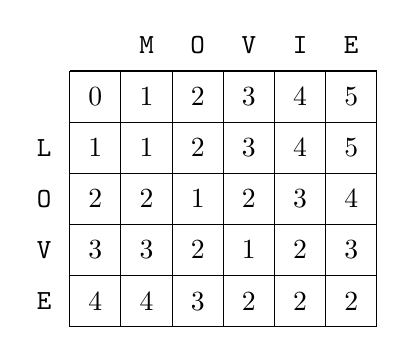
\begin{tikzpicture}[scale=.65]
  \begin{scope}
    %\fill [color=lightgray] (5, -3) rectangle (6, -4);
    \draw (1, -1) grid (7, -6);
    
    \node at (0.5,-2.5) {\texttt{L}};
    \node at (0.5,-3.5) {\texttt{O}};
    \node at (0.5,-4.5) {\texttt{V}};
    \node at (0.5,-5.5) {\texttt{E}};

    \node at (2.5,-0.5) {\texttt{M}};
    \node at (3.5,-0.5) {\texttt{O}};
    \node at (4.5,-0.5) {\texttt{V}};
    \node at (5.5,-0.5) {\texttt{I}};
    \node at (6.5,-0.5) {\texttt{E}};

    \node at (1.5,-1.5) {$0$};
    \node at (1.5,-2.5) {$1$};
    \node at (1.5,-3.5) {$2$};
    \node at (1.5,-4.5) {$3$};
    \node at (1.5,-5.5) {$4$};
    \node at (2.5,-1.5) {$1$};
    \node at (2.5,-2.5) {$1$};
    \node at (2.5,-3.5) {$2$};
    \node at (2.5,-4.5) {$3$};
    \node at (2.5,-5.5) {$4$};
    \node at (3.5,-1.5) {$2$};
    \node at (3.5,-2.5) {$2$};
    \node at (3.5,-3.5) {$1$};
    \node at (3.5,-4.5) {$2$};
    \node at (3.5,-5.5) {$3$};
    \node at (4.5,-1.5) {$3$};
    \node at (4.5,-2.5) {$3$};
    \node at (4.5,-3.5) {$2$};
    \node at (4.5,-4.5) {$1$};
    \node at (4.5,-5.5) {$2$};
    \node at (5.5,-1.5) {$4$};
    \node at (5.5,-2.5) {$4$};
    \node at (5.5,-3.5) {$3$};
    \node at (5.5,-4.5) {$2$};
    \node at (5.5,-5.5) {$2$};
    \node at (6.5,-1.5) {$5$};
    \node at (6.5,-2.5) {$5$};
    \node at (6.5,-3.5) {$4$};
    \node at (6.5,-4.5) {$3$};
    \node at (6.5,-5.5) {$2$};
  \end{scope}
\end{tikzpicture}
\end{center}

Donji desni kut tablice
nam govori da je udaljenost uređivanja između
\texttt{LOVE} i \texttt{MOVIE} jednaka 2.
Tablica također pokazuje kako konstruirati
najkraći slijed operacija uređivanja.
U ovom slučaju put je sljedeći:

\begin{center}
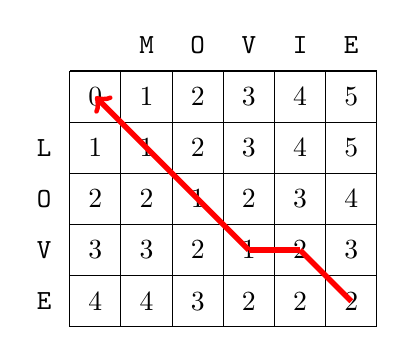
\begin{tikzpicture}[scale=.65]
  \begin{scope}
    \draw (1, -1) grid (7, -6);
    
    \node at (0.5,-2.5) {\texttt{L}};
    \node at (0.5,-3.5) {\texttt{O}};
    \node at (0.5,-4.5) {\texttt{V}};
    \node at (0.5,-5.5) {\texttt{E}};

    \node at (2.5,-0.5) {\texttt{M}};
    \node at (3.5,-0.5) {\texttt{O}};
    \node at (4.5,-0.5) {\texttt{V}};
    \node at (5.5,-0.5) {\texttt{I}};
    \node at (6.5,-0.5) {\texttt{E}};

    \node at (1.5,-1.5) {$0$};
    \node at (1.5,-2.5) {$1$};
    \node at (1.5,-3.5) {$2$};
    \node at (1.5,-4.5) {$3$};
    \node at (1.5,-5.5) {$4$};
    \node at (2.5,-1.5) {$1$};
    \node at (2.5,-2.5) {$1$};
    \node at (2.5,-3.5) {$2$};
    \node at (2.5,-4.5) {$3$};
    \node at (2.5,-5.5) {$4$};
    \node at (3.5,-1.5) {$2$};
    \node at (3.5,-2.5) {$2$};
    \node at (3.5,-3.5) {$1$};
    \node at (3.5,-4.5) {$2$};
    \node at (3.5,-5.5) {$3$};
    \node at (4.5,-1.5) {$3$};
    \node at (4.5,-2.5) {$3$};
    \node at (4.5,-3.5) {$2$};
    \node at (4.5,-4.5) {$1$};
    \node at (4.5,-5.5) {$2$};
    \node at (5.5,-1.5) {$4$};
    \node at (5.5,-2.5) {$4$};
    \node at (5.5,-3.5) {$3$};
    \node at (5.5,-4.5) {$2$};
    \node at (5.5,-5.5) {$2$};
    \node at (6.5,-1.5) {$5$};
    \node at (6.5,-2.5) {$5$};
    \node at (6.5,-3.5) {$4$};
    \node at (6.5,-4.5) {$3$};
    \node at (6.5,-5.5) {$2$};

    \path[draw=red,thick,-,line width=2pt] (6.5,-5.5) -- (5.5,-4.5);
    \path[draw=red,thick,-,line width=2pt] (5.5,-4.5) -- (4.5,-4.5);
    \path[draw=red,thick,->,line width=2pt] (4.5,-4.5) -- (1.5,-1.5);
  \end{scope}
\end{tikzpicture}
\end{center}

Posljednji znakovi nizova \texttt{LOVE} i \texttt{MOVIE}
su jednaki, pa je udaljenost uređivanja između njih
jednaka udaljenosti uređivanja između \texttt{LOV} i \texttt{MOVI}.
Jednom operacijom uređivanja možemo ukloniti
znak \texttt{I} iz \texttt{MOVI}.
Dakle, udaljenost uređivanja je za jedan veća od
udaljenosti uređivanja između \texttt{LOV} i \texttt{MOV}, itd.

\section{Brojanje popločavanja}

Ponekad su stanja rješenja dinamičkog programiranja
složenija od fiksnih kombinacija brojeva.
Kao primjer,
razmotrimo zadatak izračunavanja
broja različitih načina da se
mreža $n \times m$ popuni pločicama
veličine $1 \times 2$ i $2 \times 1$.
Na primjer, jedno valjano rješenje
za mrežu $4 \times 7$ je
\begin{center}
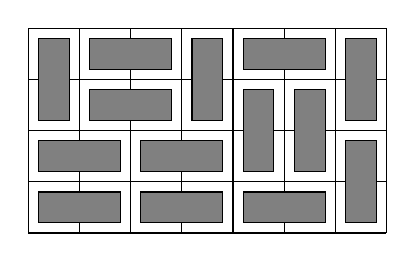
\begin{tikzpicture}[scale=.65]
    \draw (0,0) grid (7,4);
    \draw[fill=gray] (0+0.2,0+0.2) rectangle (2-0.2,1-0.2);
    \draw[fill=gray] (2+0.2,0+0.2) rectangle (4-0.2,1-0.2);
    \draw[fill=gray] (4+0.2,0+0.2) rectangle (6-0.2,1-0.2);
    \draw[fill=gray] (0+0.2,1+0.2) rectangle (2-0.2,2-0.2);
    \draw[fill=gray] (2+0.2,1+0.2) rectangle (4-0.2,2-0.2);
    \draw[fill=gray] (1+0.2,2+0.2) rectangle (3-0.2,3-0.2);
    \draw[fill=gray] (1+0.2,3+0.2) rectangle (3-0.2,4-0.2);
    \draw[fill=gray] (4+0.2,3+0.2) rectangle (6-0.2,4-0.2);

    \draw[fill=gray] (0+0.2,2+0.2) rectangle (1-0.2,4-0.2);
    \draw[fill=gray] (3+0.2,2+0.2) rectangle (4-0.2,4-0.2);
    \draw[fill=gray] (6+0.2,2+0.2) rectangle (7-0.2,4-0.2);
    \draw[fill=gray] (4+0.2,1+0.2) rectangle (5-0.2,3-0.2);
    \draw[fill=gray] (5+0.2,1+0.2) rectangle (6-0.2,3-0.2);
    \draw[fill=gray] (6+0.2,0+0.2) rectangle (7-0.2,2-0.2);

\end{tikzpicture}
\end{center}
a ukupan broj rješenja je 781.

Zadatak se može riješiti dinamičkim programiranjem
prolaskom kroz mrežu redak po redak.
Svaki redak u rješenju može se prikazati kao
znakovni niz koji sadrži $m$ znakova iz skupa
$\{\sqcap, \sqcup, \sqsubset, \sqsupset \}$.
Na primjer, gornje rješenje sastoji se od četiri retka
koji odgovaraju sljedećim znakovnim nizovima:
\begin{itemize}
\item
$\sqcap \sqsubset \sqsupset \sqcap \sqsubset \sqsupset \sqcap$
\item
$\sqcup \sqsubset \sqsupset \sqcup \sqcap \sqcap \sqcup$
\item
$\sqsubset \sqsupset \sqsubset \sqsupset \sqcup \sqcup \sqcap$ 
\item
$\sqsubset \sqsupset \sqsubset \sqsupset \sqsubset \sqsupset \sqcup$
\end{itemize}

Neka $\texttt{count}(k,x)$ označava broj načina da se
konstruira rješenje za retke $1 \ldots k$
mreže tako da znakovni niz $x$ odgovara retku $k$.
Ovdje je moguće koristiti dinamičko programiranje,
jer je stanje retka ograničeno
samo stanjem prethodnog retka.

Rješenje je valjano ako redak $1$ ne sadrži
znak $\sqcup$,
redak $n$ ne sadrži znak $\sqcap$,
i svi su uzastopni redci \emph{kompatibilni}.
Na primjer, redci
$\sqcup \sqsubset \sqsupset \sqcup \sqcap \sqcap \sqcup$ i
$\sqsubset \sqsupset \sqsubset \sqsupset \sqcup \sqcup \sqcap$ 
su kompatibilni, dok redci
$\sqcap \sqsubset \sqsupset \sqcap \sqsubset \sqsupset \sqcap$ i
$\sqsubset \sqsupset \sqsubset \sqsupset \sqsubset \sqsupset \sqcup$
nisu kompatibilni.

Budući da se redak sastoji od $m$ znakova i postoje
četiri izbora za svaki znak, broj različitih
redaka je najviše $4^m$.
Stoga je vremenska složenost rješenja
$O(n 4^{2m})$ jer za svaki redak možemo proći kroz
$O(4^m)$ mogućih stanja,
a za svako stanje postoji $O(4^m)$
mogućih stanja za prethodni redak.
U praksi je dobra ideja rotirati mrežu
tako da kraća stranica ima duljinu $m$,
jer faktor $4^{2m}$ dominira vremenskom složenošću.

Rješenje je moguće učiniti efikasnijim
korištenjem kompaktnijeg prikaza redaka.
Pokazuje se da je dovoljno znati koji
stupci prethodnog retka sadrže gornji kvadrat
okomite pločice.
Stoga redak možemo prikazati koristeći samo znakove
$\sqcap$ i $\Box$, gdje je $\Box$ kombinacija
znakova
$\sqcup$, $\sqsubset$ i $\sqsupset$.
Uz taj prikaz postoji samo
$2^m$ različitih redaka i vremenska složenost je
$O(n 2^{2m})$.

Kao završnu napomenu, postoji i iznenađujuća izravna formula
za izračunavanje broja popločavanja\footnote{Iznenađujuće,
ovu su formulu 1961. otkrila dva istraživačka tima \cite{kas61,tem61}
koja su radila neovisno.}:
\[ \prod_{a=1}^{\lceil n/2 \rceil} \prod_{b=1}^{\lceil m/2 \rceil} 4 \cdot (\cos^2 \frac{\pi a}{n + 1} + \cos^2 \frac{\pi b}{m+1})\]
Ova formula je vrlo efikasna, jer izračunava
broj popločavanja u $O(nm)$ vremenu,
ali budući da je odgovor proizvod realnih brojeva,
problem pri korištenju formule jest
kako točno pohraniti međurezultate.


